\documentclass[12pt]{article}
\usepackage{graphicx}
\usepackage{hyperref}
\usepackage[top=2.75in, left=1in, right=1in, bottom=0.25in]{geometry}
\usepackage[utf8]{inputenc}
\usepackage[english]{babel}
\usepackage{fancyhdr}
\usepackage[utf8]{inputenc}
\usepackage{listings}
\usepackage{color}
\usepackage[final]{pdfpages}
\usepackage{multirow}
\usepackage{array}
\usepackage{caption}
\usepackage{subcaption}

\definecolor{codegreen}{rgb}{0,0.6,0}
\definecolor{codegray}{rgb}{0.5,0.5,0.5}
\definecolor{codepurple}{rgb}{0.58,0,0.82}
\definecolor{backcolour}{rgb}{0.95,0.95,0.92} 
\lstdefinestyle{mystyle}{
    backgroundcolor=\color{backcolour},   
    commentstyle=\color{codegreen},
    keywordstyle=\color{magenta},
    numberstyle=\tiny\color{codegray},
    stringstyle=\color{codepurple},
    basicstyle=\footnotesize,
    breakatwhitespace=false,         
    breaklines=true,                 
    captionpos=b,                    
    keepspaces=true,                 
    numbers=left,                    
    numbersep=5pt,                  
    showspaces=false,                
    showstringspaces=false,
    showtabs=false,                  
    tabsize=2
} 
\lstset{style=mystyle}

\setlength{\parindent}{4em}
\setlength{\parskip}{1em}
\pagestyle{fancy}
\fancyhf{}
\rhead{Assignment 9}
\lhead{Huan Huang}
\renewcommand{\headrulewidth}{0.4pt}
\renewcommand{\footrulewidth}{0.4pt}
\rfoot{Page \thepage}


\begin{document}
\begin{titlepage}
	\begin{center}
	\Huge{Web Science cs532-s16}\\
	[0.25in]
	\textsc{\Large Assignment 9 Report}\\
	\textsc{\normalsize Dr. Michael L. Nelson}\\
	[4.25in]
	\textsc{\normalsize By: Huan Huang}\\
	\large 04/22/2016\\
	
	
	\end{center}
\end{titlepage}
\newpage

\newgeometry{margin=1in}


\section*{Problem 1}


\begin{verbatim}
Choose a blog or a newsfeed (or something similar with an Atom
or RSS feed).  Every student should do a unique feed, so please
"claim" the feed on the class email list (first come, first served).
It should be on a topic or topics of which you are qualified to
provide classification training data.  Find something with at least
100 entries (or items if RSS).

Create between four and eight different categories for the entries
in the feed:

examples: 

work, class, family, news, deals

liberal, conservative, moderate, libertarian

sports, local, financial, national, international, entertainment

metal, electronic, ambient, folk, hip-hop, pop

Download and process the pages of the feed as per the week 12 
class slides.
\end{verbatim}

\subsection*{Answer}
I took me a long time to find a web page with over 100 RSS feeds. I eventually used PlayStation's RSS feeds for movies, which has over 10 thousand feeds. I downloaded and save the feeds with the curl -o command and saved it as psMovies.xml. Next, I picked out the categories for classifying the entries, which are:

\noindent
action - a film genre in which the characters are thrust into a series of challenges that involve physical feats, extended fight scenes, violence, and frantic chases.

\noindent
comedy - a genre of film in which the main emphasis is on humour. These films are designed to make the audience laugh through amusement and most often work by exaggerating characteristics for humorous effect. Films in this style traditionally have a happy ending (black comedy being an exception).

\noindent
scifi - a film genre that uses science fiction: speculative, fictional science-based depictions of phenomena that are not fully accepted by mainstream science, such as extraterrestrial life forms, alien worlds, extrasensory perception and time travel, along with futuristic elements such as spacecraft, robots, cyborgs, interstellar space travel or other technologies. Science fiction films have often been used to focus on political or social issues, and to explore philosophical issues like the human condition.

\noindent
horror - unsettling films designed to frighten and panic, cause dread and alarm, and to invoke our hidden worst fears, often in a terrifying, shocking finale, while captivating and entertaining us at the same time in a cathartic experience.

\noindent
romance - romantic love stories recorded in visual media for broadcast in theaters and on television that focus on passion, emotion, and the affectionate romantic involvement of the main characters and the journey that their genuinely strong, true and pure romantic love takes them through dating, courtship or marrige. Romance films make the romantic love story or the search for strong and pure love and romance the main plot focus.

\noindent
other - other movie genres that are not included above.\\
(I copied the movie genre definitions from WIKIPEKIA)



\section*{Problem 2}

\begin{verbatim}
Manually classify the first 50 entries, and then classify (using
the fisher classifier) the remaining 50 entries. 

Create a table with the title, predicted category, actual category,
and cprob() and fisherprob() for the actual category.
\end{verbatim}

\subsection*{Answer}
I copy and modified the files docclass.py and feedfilter.py to solve this problem. The program feedfilter.py reads and parse the entries from psMovies.xml. And for each of the top 50 entries, I enter an actual classification which is use to call the classifier.train() function in docclass.py. This is used to train the classifier and enables it to make predictions of the category of the movies based on my input. I also get the fisher's conditional probability by calling the classifier.cprob() and classifier.fisherprob() functions, the actual category is to those functions to calculate the probabilities .
\pagebreak

\begin{figure}[h!]
\centering
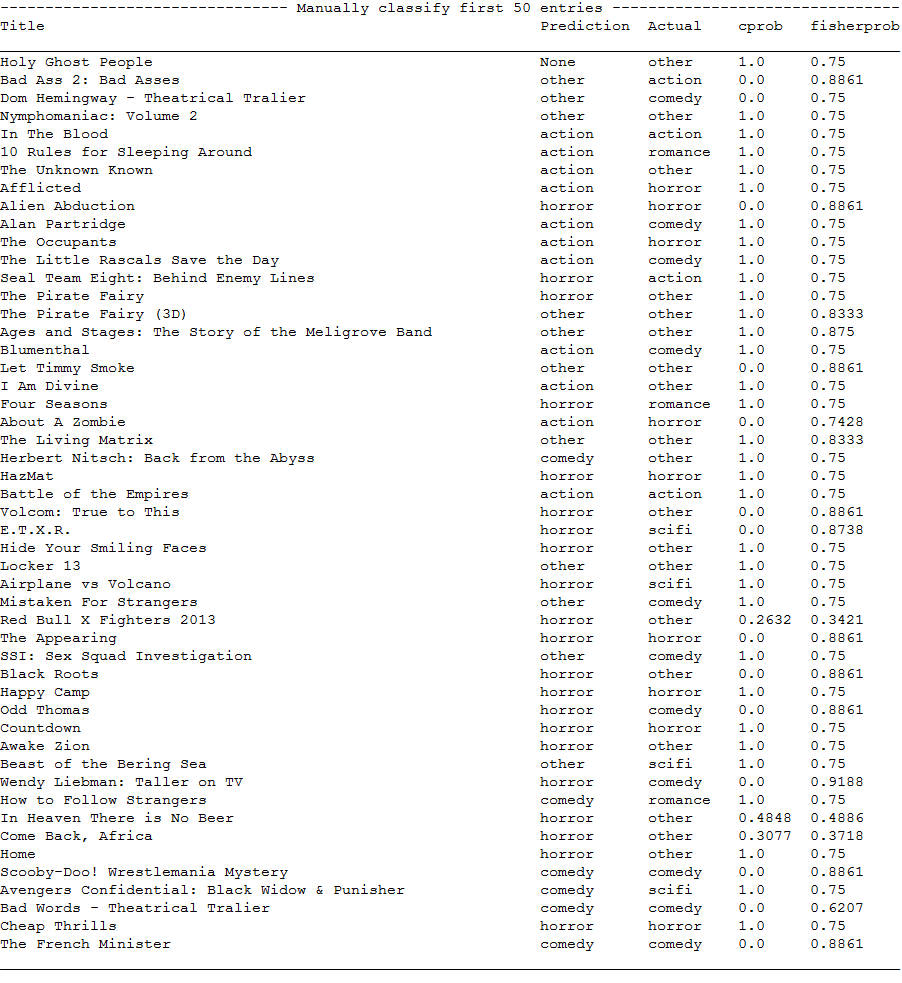
\includegraphics[width=6.5in]{top50.png}
\end{figure}

\begin{figure}[h!]
\centering
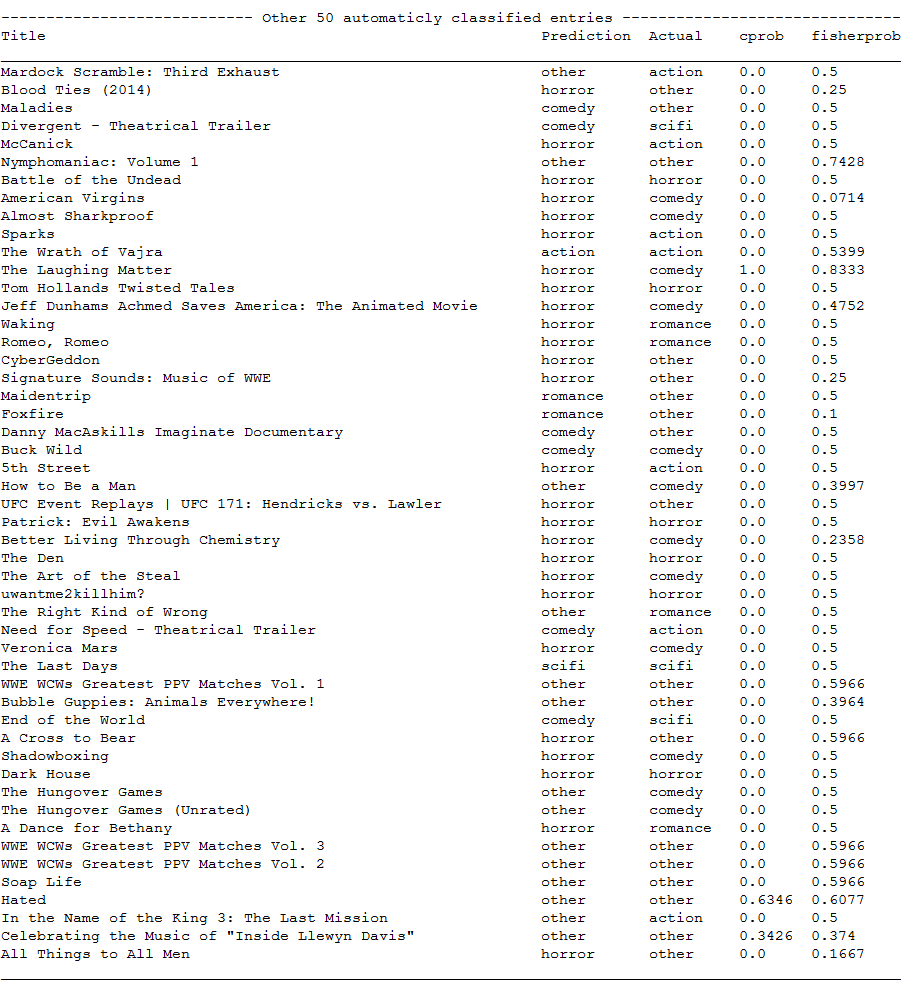
\includegraphics[width=6.5in]{bot50.png}
\end{figure}
\pagebreak

\lstinputlisting[language=python]{feedfilter.py}
\lstinputlisting[language=python]{docclass.py}

\section*{Problem 3}

Assess the performance of your classifier in each of your
categories by computing precision, recall, and F-measure. 

\subsection*{Answer}
In order to calculate the precision, recall, and F-measures. I first have to get the false positive, false negative, and true positive of the predictions. Where the prediction matched my actual input for each category is the true positive for each category. The false positive and false negative is obtained by subtracting the TP from predicted and actual counts of each category. Then use the formulas from lecture slides to calculated the precision, recall, and F-measures.

\begin{figure}[h!]
\centering
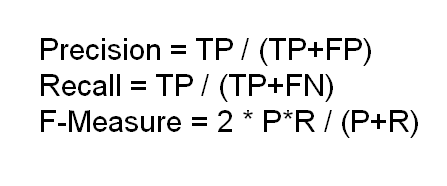
\includegraphics[width=2in]{formulas.png}
\end{figure}

\begin{center}
\begin{tabular}{ | m{0.8in} | m{0.3in}| m{0.3in} | m{0.3in} | m{0.8in} | m{0.5in} | m{1in} |} 
\hline
Categories & FP & FN & TP & Precision & Recall & F-measure \\
\hline
Action & 10 & 7 & 3 & 0.23 & 0.3 & 0.26 \\ 
\hline
Comedy & 8 & 19 & 4 & 0.33 & 0.17 & 0.22 \\ 
\hline
Horror & 35 & 3 & 12 & 0.26 & 0.8 & 0.39 \\ 
\hline
Other & 10 & 24 & 14 & 0.58 & 0.37 & 0.45 \\ 
\hline
Romance & 2 & 7 & 0 & 0 & 0 & 0 \\ 
\hline
Scifi & 0 & 6 & 1 & 1 & 0.14 & 0.25 \\ 
\hline
\end{tabular}
\end{center}

Based on the result, the classifier did not perform well at all, but it was expected, since I only trained it with 50 entries.

\end{document}